%! Author = ashutosh
%! Date = 4/20/22

\documentclass[english]{sobraep}
\usepackage[english]{babel}
\usepackage{float}
\usepackage{amsmath}
\usepackage{graphicx}
\usepackage{caption}
\usepackage{subcaption}
\usepackage{hyperref}
\hypersetup{
    colorlinks=true,
    citecolor=green,
    linkcolor=blue,
    filecolor=cyan,      
    urlcolor=magenta,
    }
\usepackage[utf8]{inputenc}
\usepackage{fancyhdr}
\usepackage{listings}


\title{Learning Relational Bias from Differential Scenes in Deep Reinforcement Learning}


\author{Ashutosh Tiwari\\
	\normalsize ashutiwa@iu.edu
}

\pagestyle{fancy}
\fancyhf{}
\lhead{Presented as a project for RL (B 659 Spring 2022)}
\rfoot{Page \thepage}
\begin{document}
\maketitle


\begin{abstract}
    In this work we introduce a novel way to build relational reasoning between different entities in a scene by observing changes in the scene in the last step for on-policy reinforcement algorithms. We did a lot of experiments and found that even though this is a computationally efficient way to process difference in scenes (as compared to original image), it gives comparable results to ones proposed before.
    
    This work uses A2C algorithm ~\cite{DBLP:journals/corr/abs-1802-01561} to optimize value function and predict actions, however we propose that there is nothing stopping us to try A3C ~\cite{DBLP:journals/corr/MnihBMGLHSK16} or any other similar algorithm. However that was not covered as part of this project.
    
    When we started our initial goal was to explore the affects of inducing relational inductive bias in a deep RL, high dimensional action space setting, but as the project progressed we realized that just using movement to represent state, specially in cases where number of agents are manageable gives much better results as compared to approaches which do not do the same.
    
    This project should be viewed as a continuation of works of ~\cite{zambaldi2018deep} in the sense that it extends it's applicability in three tangential ways \begin{itemize}
	    \item Authors explore this idea in a very low dimensional action space ( StarCraft II action space $\sim 100$), while in case of Street Fighter it is $2^{12}$.
	    \item We propose that this idea works even when we only use the changes in scene, which is computationally much more efficient since only a handful of pixels have changed.
	    \item This is a method to be used in an online training algorithm as opposed to what authors use in their literature.
	\end{itemize}  
\end{abstract}
\noindent \textbf{Keywords.} Deep Reinforcement Learning, Attention, Relational Inductive Biases

%~~~~~~~~~~~~~~~~~~~~~~~~~~~~~~~~~~~~~~~~
%Sections
%~~~~~~~~~~~~~~~~~~~~~~~~~~~~~~~~~~~~~~~~

%Introduction

\section{INTRODUCTION}

	Initially deep learning evolved as a way of end to end solution which takes raw/unstructured data and outputs result. In most of cases particularly in case of large state spaces they have enjoyed good results, because of these models were quite expressive, flexible to train and could model the environment better than previous methods. 
	
	As our understanding of these models grew, we started in some regularization ~\cite{DBLP:journals/corr/abs-1207-0580} or making sure that intermediate layers learn some structured patterns ~\cite{DBLP:journals/corr/RonnebergerFB15}.
	
	Similarly, in case of reinforcement learning for a very long time most of works ( for example ~\cite{DBLP:journals/corr/GarneloAS16}) explored structured deep learning approaches, most of which were required explicitly hand designed formulations of these relations between entities currently in action.  Relational Inductive Biases have been explored in many approaches in past.  of which most notable and famous are ~\cite{DBLP:journals/corr/abs-1806-01261} and ~\cite{zambaldi2018deep}. Both of these works were the first to establish importance of learning relations between different entities in a reinforcement learning setting.
	
\begin{figure}[H]
	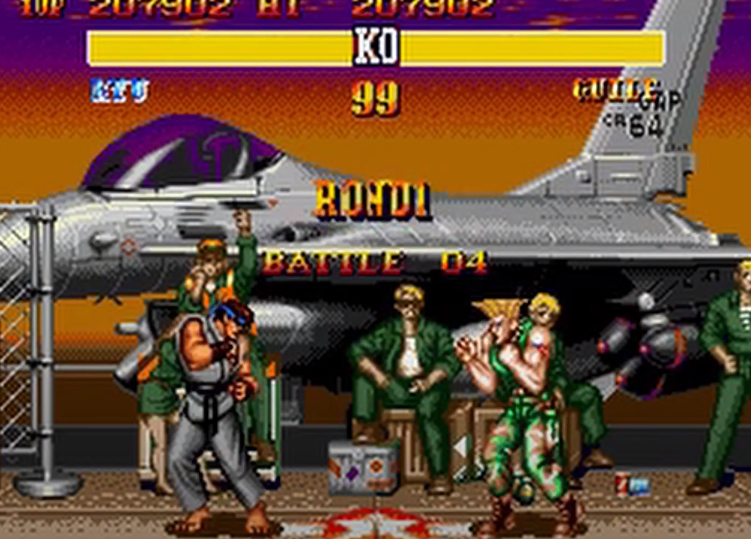
\includegraphics[scale=.32]{game.png}
	\centering
	\caption{A still from game}
	\label{fig:fig1}
\end{figure}	


\section{ENVIRONMENT}

Custom \href{https://github.com/thunderock/BiasNet/blob/master/environment.py}{environment} was written on top of ~\cite{nichol2018retro}. This environment supports different settings for different quality (size, resolution etc) observations (images) and whether to capture changes in scene (which we call differential scenes repeatedly). This also define the reward structure, which is $$R(a, s) = \nabla H(s) -\nabla EH(s) + IFWON$$ where $H(s)$ is the current health, thus $\nable H(s)=H(s) - H(s - 1)$ ranges from $[-176, 0]$, $EH(s)$ is the enemy health $\nabla EH(s) = EH(s) - EH(s-1)$ ranges from $[-176, 0]$ and $IFWON$ is either $10000$ or $-10000$ depending on whether agent was able to win the game in the end or not. 

This reward structure was a result of numerous experiments and trial and error. This was found to be the most satisfactory and seems sufficient for the purpose of goal we are trying to achieve here.

The game structure and rules themselves are very simple. An agent and a character from the game fight for maximum of three rounds and however wins the most number of rounds wins the game. This constitutes an episode. if a player first two games, then also game ends at that point.

Action space is $2^{12}$ i.e. $12$ digit multibinary. There is no other observation provided to the model other than $84\times84\times1$ dimensional image output of the scene.

\begin{figure*}
	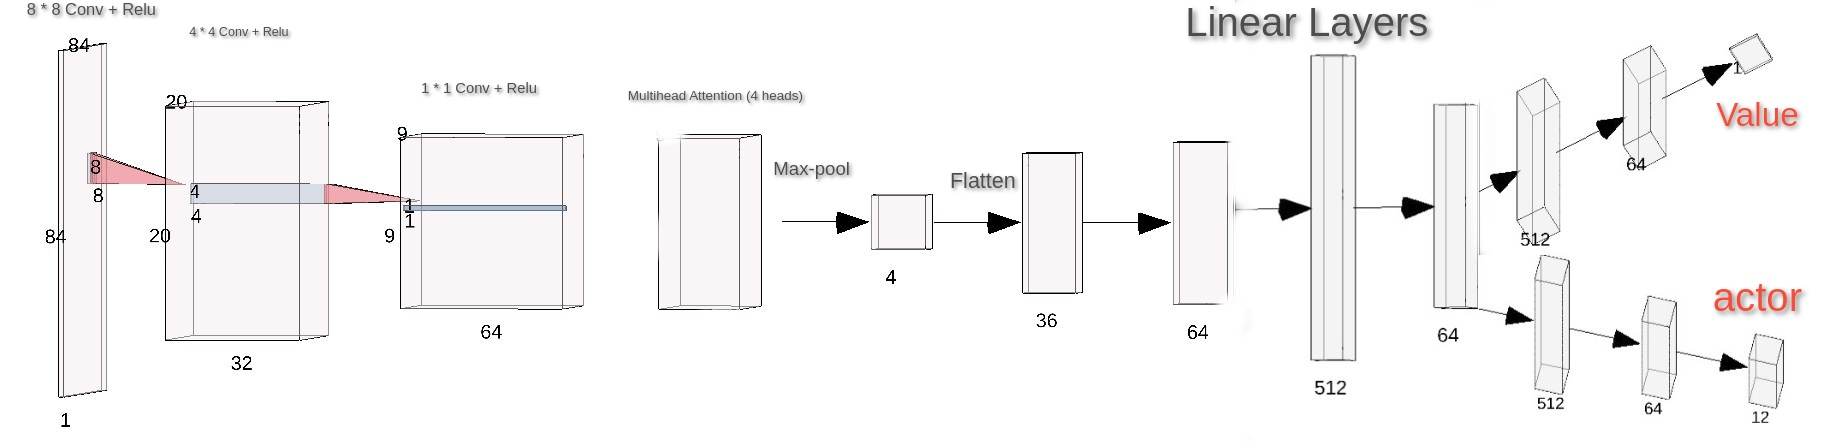
\includegraphics[width=\textwidth]{relational.jpg}
	\centering
	\caption{Relational Architecture}
	\label{fig:fig2}
\end{figure*}	

\begin{figure*}
	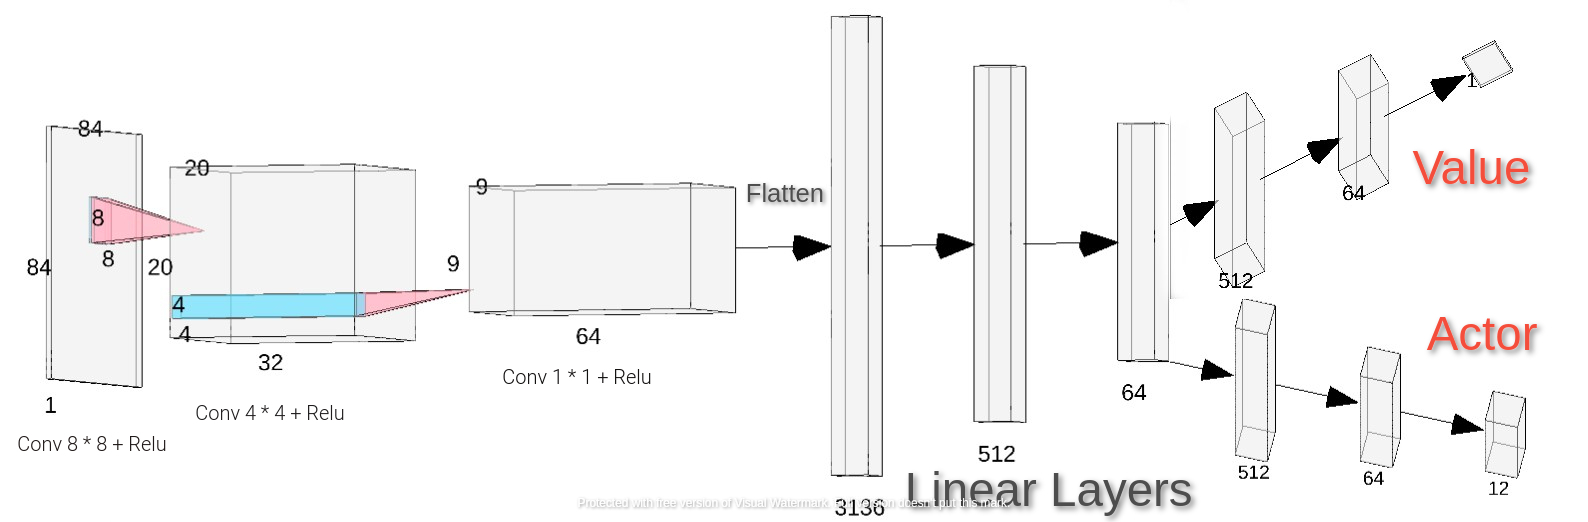
\includegraphics[width=\textwidth]{non_relational.jpeg}
	\centering
	\caption{Non Relational Architecture}
	\label{fig:fig3}
\end{figure*}	

\section{AGENT ARCHITECTURE}
Code for this project has been made available \href{https://github.com/thunderock/BiasNet/}{here}. It uses ~\cite{NEURIPS2019_9015} and ~\cite{stable-baselines3} as backbone of the code. Custom modules (feature extractors, policy networks, value models etc.) are part of the repository. Network takes a $84\times84\times1$ grayscale image, which is either a movement in scene (current state - previous state) or the current scene depending on the model under consideration.

Block diagrams show the model architecture for both the relation model in ~\ref{fig:fig2} and non relational baseline in ~\ref{fig:fig3} respectively. Number of heads used for Multihead Attention ~\cite{DBLP:journals/corr/VaswaniSPUJGKP17} is $4$. For more details of architecture please follow this \href{https://github.com/thunderock/BiasNet/blob/master/model_architecture.ipynb}{link} which is generated using named parameters in policy network module.

Parameters used to train all models were 
\begin{lstlisting}
'gamma': 0.8074138106735396, 
'learning_rate': 0.0001, 
'gae_lambda': 0.8787060424267222
\end{lstlisting}
These were also result of extensive experiments, but yes since these models were trained for a very large number of episodes, hyper-parameter tuning at a large scale was difficult. At the end we decided to settle for callback approach where we were evaluating model at every $30K$ steps and then saving same. More details regarding the training procedure and methodology in next section.


\section{EXPERIMENTS AND RESULTS}

Each model is trained for 5M episodes with a batch size of $256$. Hyper parameters to train models were figured out over the course of project. To derive some intuition on what could be the best, we looked at these ~\ref{fig:fig6} and ~\ref{fig:fig7}. These plots were result of training on an entirely different reward structure, but we think that on a very high level it is wise to use these as baselines. For non relational baselines they was kept the same. We see that before starting to overfit, the relational agent which is trained on movements achieves a higher mean reward much early than all other methods. A callback is used to monitor the training model every $30K$ episodes and if it is better than the previous model it is stored to be used for prediction.

All experiments can be found in \href{https://github.com/thunderock/BiasNet/tree/master/experiments}{experiments directory} in the root folder of the project. These include tuning results (which were done using optuna), tensorboard logs, final recordings and trained models. All of them are in obvious directory structure which are aptly named.

\begin{figure}
	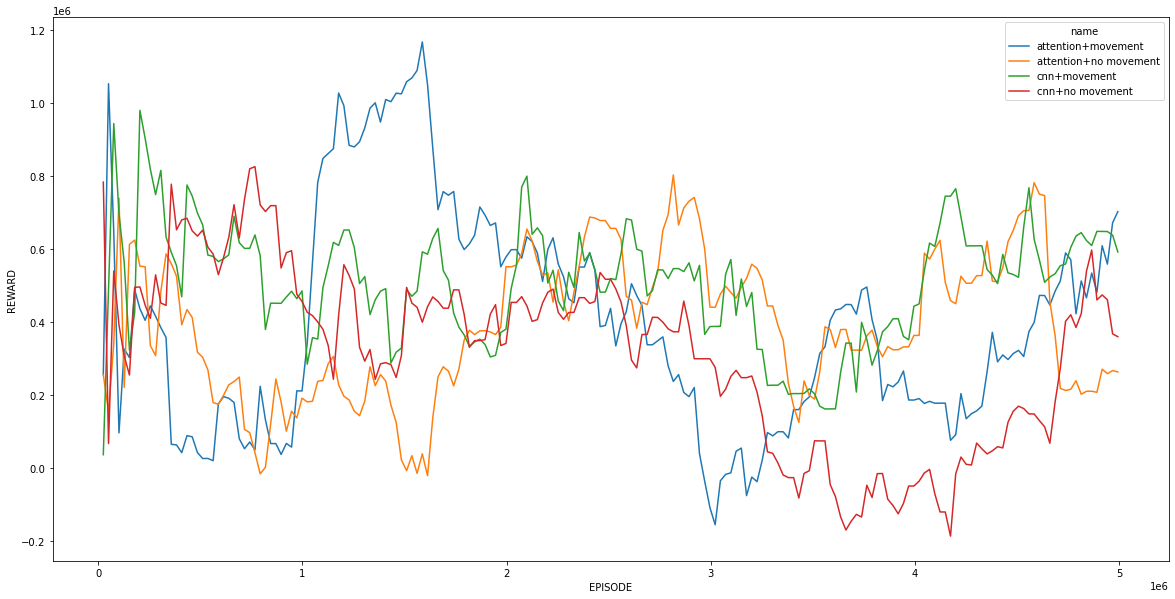
\includegraphics[width=3in, height=3in]{training.png}
	\centering
	\caption{Average Rollout Reward during training}
	\label{fig:fig4}
\end{figure}


\begin{figure}
	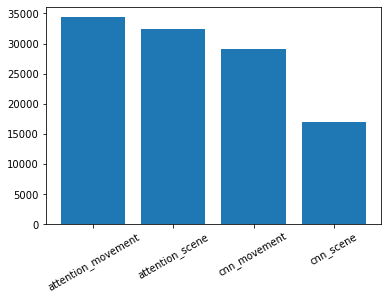
\includegraphics[width=3in]{scores.png}
	\centering
	\caption{Model Scores}
	\label{fig:fig5}
\end{figure}
\begin{figure}
	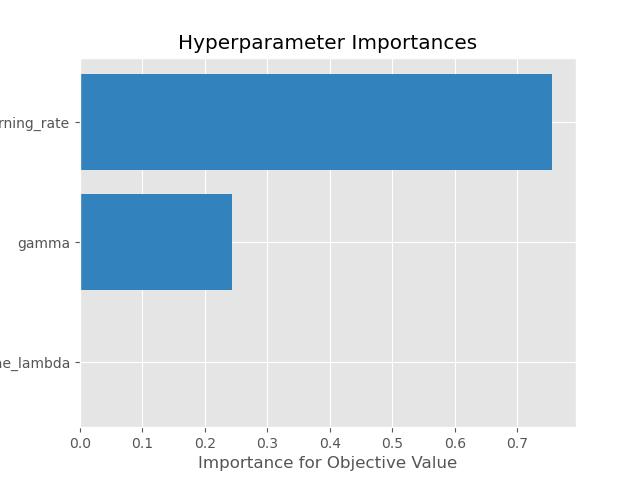
\includegraphics[width=3in, height=3in]{plot_param_importances.png}
	\centering
	\caption{Hyper-parameters' importance}
	\label{fig:fig6}
\end{figure}
\begin{figure}
	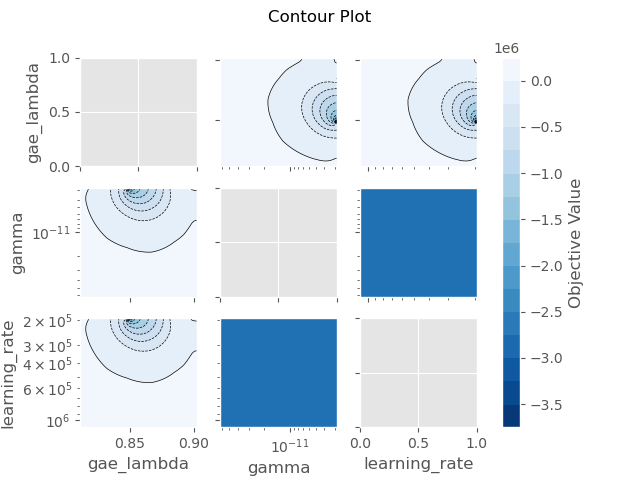
\includegraphics[width=3in, height=3in]{biased_movement_contour.png}
	\centering
	\caption{Contour plot for hyper-parameters}
	\label{fig:fig7}
\end{figure}

There were a few challenges encountered. We are listing those down below. Some of the ways of improve on these are discussed in future work section.

\begin{itemize}
    \item Because of large action space in this problem, training this model is very sensitive to hyper-parameters. For a very small variation in hyperparameters, results are widely different. This is also acknowledged in ~\cite{zambaldi2018deep}.
    
    \item Because it is not possible to use more than retro emulator in \href{https://github.com/openai/retro/issues/64}{one process} it was very tricky to do hyper-parameter tuning to be able to get optimal results. Only was was to run parallel python processes and optimize two models at one time.
    
\end{itemize}

\section{CONCLUSION AND FUTURE WORK}

It was very easy to point out that using relational agent in this case doesn't not result in very high improvements in evaluation results when compared to the computational overheads and complexity it brings to the system, at least in this case. This was the fact we set out to prove in the beginning. But it does provide little better results. Major find was the use of scene differences in the training itself. This gave a lot of improvement as can be seen ~\ref{fig:fig5}. This plot is generated from the selected trained models in each category.

I think there were a lot of things I could've done better. First I realized that my network was very small as compared to  ~\cite{zambaldi2018deep}, and this was an online learning algorithm as compared to an offline version they used in their paper. It required 100 workers to be trained in parallel and they used two different networks. In my case use of a small network was a cautious decision to keep the network size contained to be able to train model on the infrastructure which was at my disposal. Also as you can notice in diagram ~\ref{fig:fig2}, the result of max pool is very small $4\times4$, and we're very sure that this was a bottleneck in the learning procedure. 

Authors chose box environment in their experiments which factors out all intricacies of a complex scene. In this case I tried to simplify same by capturing only the pixels which changed in current scene. But as evident from the game itself, there is a lot of background movement in observations which does not affect the outcome or progress of game in any way but is still required to be attended b the network.

I realized it little late that probably I could have some or the other way included positional embeddings. The reason I didn't include them in current implementation was that I wanted to make this comparison between pure CNN network and the attention network as similar as possible. Intuitively, it appeared to me that it should provide a boost in performance and probably it did.

Since we already know that using movements is a good idea, probably I should have tried a combination of both the observation and the changes. It would've been interesting to see the results.

\bibliographystyle{alpha}

\bibliography{ashutiwa.bib}

\end{document}

